\section*{Visualização}

Foi organizado um \textit{\textbf{Dashboard}} onde estão presentes informações sobre o negócio (compras e vendas). Este \textit{Dashboard} encontra-se organizado de forma à sua interpretação ser rápida e fácil, algo que é estritamente necessário pois os utilizadores necessitam de o visualizar e facilmente conseguirem fazer uma análise do negócio.

\subsection{Home}

A secção "Home" do \textit{Dashboard} serve para verificar dados mais gerais do negócio, a partir desta aba somos capazes de rapidamente verificar o estado do negócio.

\begin{figure}[H]
    \centering
    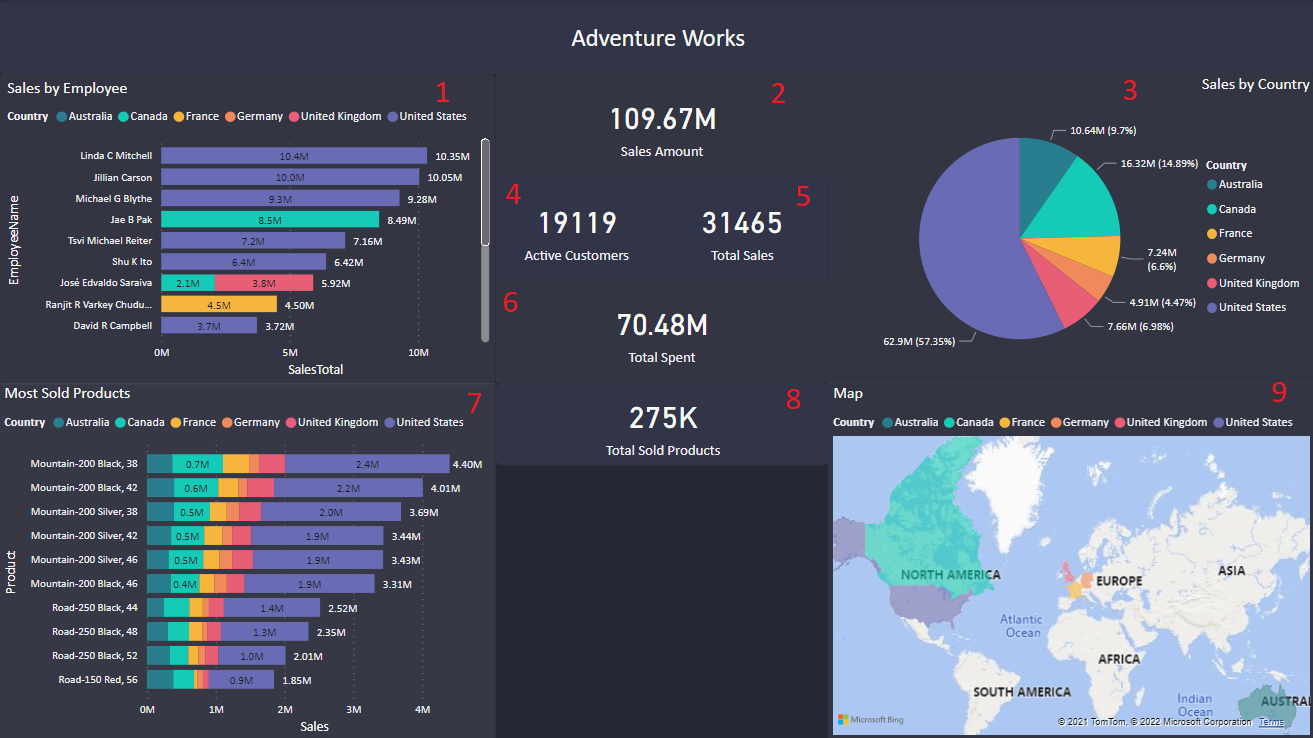
\includegraphics[scale=0.4]{images/Home.png}
    \caption{Aba "Home" do \textit{Dashboard}}
\end{figure}

\textbf{1 - Vendas por Funcionário:} Neste gráfico é possível verificar a quantidade de vendas efetuadas por funcionários (apenas aqueles que têm vendas associadas), é ainda possível verificar os países onde as vendas destes funcionários se encontram.

\textbf{2 - Quantidade de Vendas:} Este é o valor de vendas totais do negócio este valor encontra-se milhões de dólares.

\textbf{3 - Vendas por País:} Neste gráfico circular é possível verificar as vendas totais por país.

\textbf{4 - Clientes Ativos:} Este é o valor de clientes que efetuaram algum tipo de compra na empresa.

\textbf{5 - Vendas Totais:} Este é o valor total de vendas efetuadas pela empresa.

\textbf{6 - Total Gasto:} Este valor representa o valor total gasto pela empresa em compras de produtos.

\textbf{7 - Produtos mais Vendidos:} Neste gráfico é possível verificar os produtos mais vendidos em termos de valor, é ainda possível verificar o país onde estes foram vendidos.

\textbf{8 - Total Sold Products:} Este valor representa o valor total de produtos vendidos pela empresa.

\textbf{9 - Mapa:} Neste mapa estão representados os países onde a empresa fez vendas, é possível pressionar os países para verificar os dados referentes ao mesmo.
 
\subsection{Sales}

A secção "Sales" do \textit{Dashboard} serve para verificar dados sobre as vendas da empresa.


\begin{figure}[H]
    \centering
    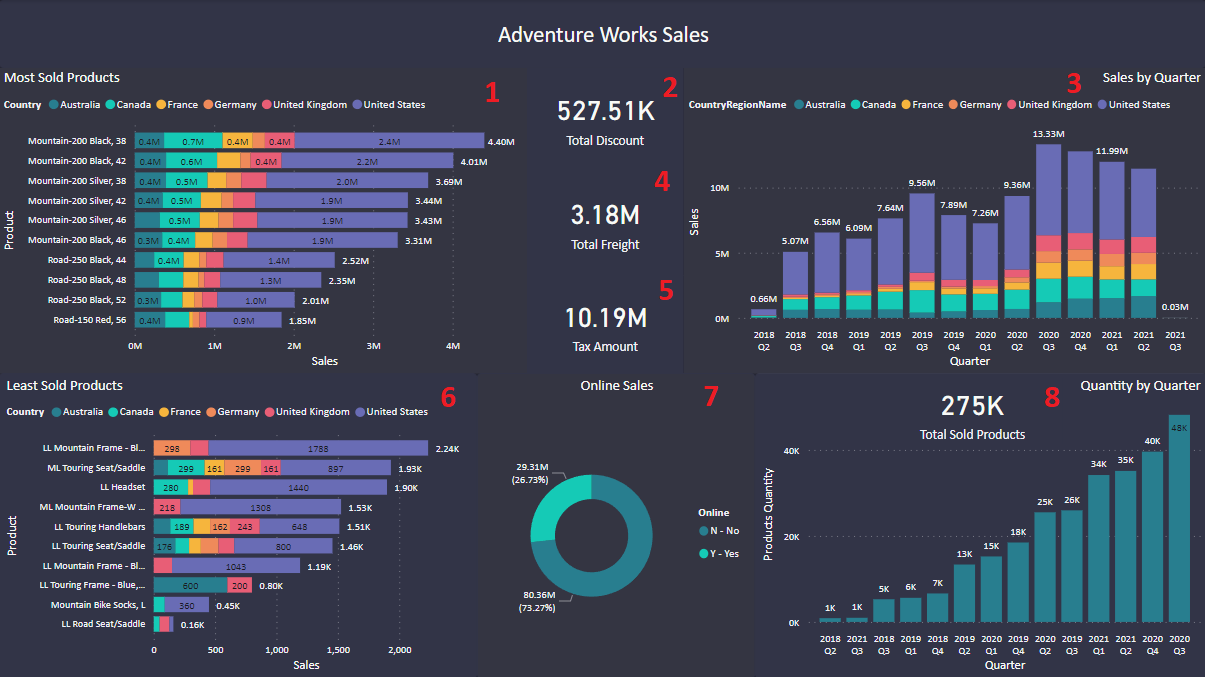
\includegraphics[scale=0.4]{images/Sales.png}
    \caption{Aba "Sales" do \textit{Dashboard}}
\end{figure}

\textbf{1 - Produtos mais Vendidos:} Neste gráfico é possível verificar os produtos mais vendidos em termos de valor, é ainda possível verificar o país onde estes foram vendidos.

\textbf{2 - Desconto total:} Este valor representa o valor monetário total em descontos das vendas.

\textbf{3 - Vendas por trimestre:} Neste gráfico é possível verificar as vendas efetuadas por trimestre, é ainda possível verificar para qual território.

\textbf{4 - Custo de envio total:} Este valor representa o total gasto em envio de produtos para venda.

\textbf{5 - Total de Taxas:} Este valor representa o total gasto taxas na venda de produtos.

\textbf{6 - Produtos menos vendidos:} Neste gráfico estão representados os produtos menos vendidos pela empresa, é ainda possível verificar para qual território.

\textbf{7 - Vendas Online:} Neste gráfico circular é possível verificar a percentagem de vendas que foram efetuadas online.

\textbf{8 - Quantidade vendida por trimestre:} Neste gráfico é possível verificar a quantidade de produtos vendida por cada trimestre. 

\newpage
\subsection{Purchases}

A secção "Purchases" do \textit{Dashboard} serve para verificar dados sobre as compras da empresa.


\begin{figure}[H]
    \centering
    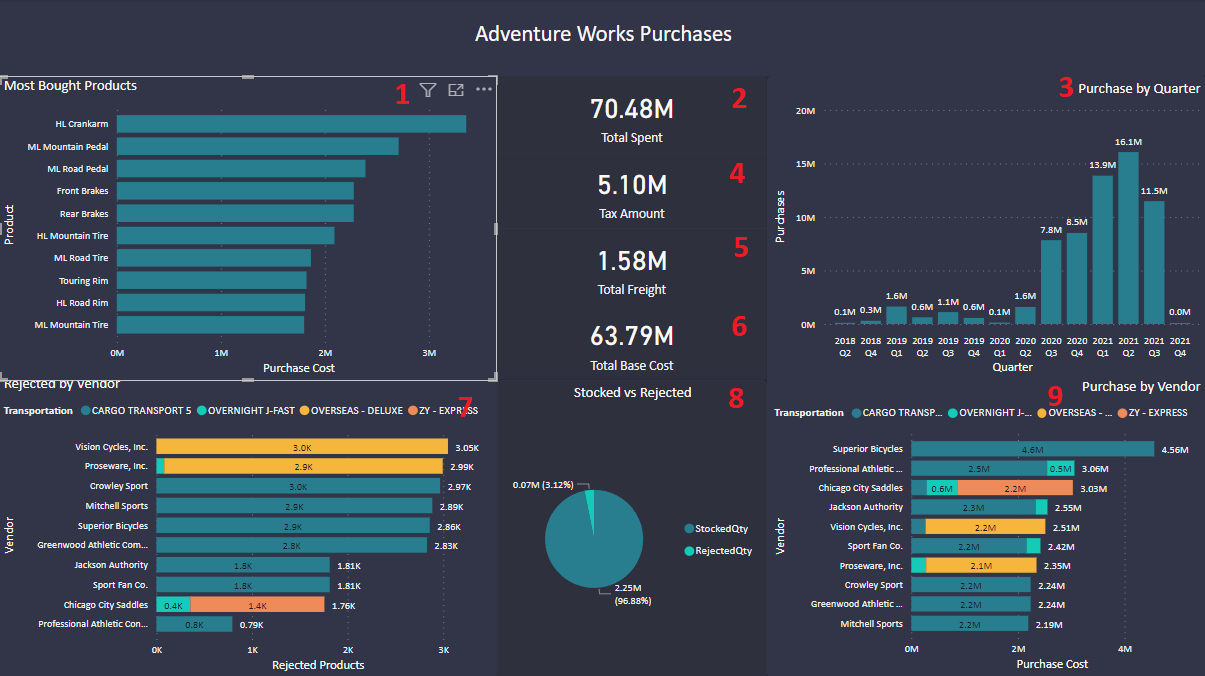
\includegraphics[scale=0.4]{images/Purchases.png}
    \caption{Aba "Purchases" do \textit{Dashboard}}
\end{figure}

\textbf{1 - Produtos mais comprados:} Neste gráfico é possível verificar os produtos que foram mais comprados pela empresa.

\textbf{2 - Total Gasto:} Este é o valor do total gasto na compra de produtos pela empresa.

\textbf{3 - Compras por trimestre:} Neste gráfico é possível verificar o dinheiro gasto em compras por cada trimestre.

\textbf{4 - Quantidade de Taxas:} Valor total gasto em taxas na compra de produtos pela empresa.

\textbf{5 - Total em transporte:} Valor total gasto no transporte de produtos comprados pela empresa.

\textbf{6 - Custo Base total:} Valor total em dinheiro antes de serem calculados impostos e preços transporte.

\textbf{7 - Rejeições por Fornecedor:} Neste gráfico é possível verificar a quantidade de produtos rejeitados por cada fornecedor, é ainda possível verificar o tipo de transporte utilizador por cada um.

\textbf{8 - Armazenado vs Rejeitado:} Neste gráfico circular é possível verificar a percentagem de produtos que foram para stock e aqueles que foram rejeitados.

\textbf{9 - Compras por fornecedor:} Neste gráfico é possível verificar verificar a quantidade de dinheiro gasto em cada fornecedor em compras, é ainda possível verificar o tipo de transporte utilizado.


